\documentclass[twocolumn]{article}
\usepackage{caption}
\usepackage[utf8]{inputenc}
\usepackage{amsmath}
\usepackage[margin=1in]{geometry}
\usepackage{changepage}
\usepackage{titling}
\usepackage{ragged2e}
\usepackage{abstract}
\usepackage{enumitem}
\usepackage{graphicx}
\usepackage{hyperref}
\renewcommand{\thesection}{\Roman{section}}
\renewcommand{\thesubsection}{(\roman{subsection})}
\renewcommand{\thesubsubsection}{\thesubsection.\arabic{subsubsection}}
\setlength\parindent{5pt}
\setlength{\columnsep}{1cm}

\begin{document}

\twocolumn[
\begin{@twocolumnfalse}
\title{\Large{\textbf{Optical Pumping of $Rb^{85}$ and $Rb^{87}$}}}
\author{Herbert D. Ludowieg}
\setlength{\droptitle}{-0.65in}
\maketitle
\begin{onecolabstract}
\justify
Optical Pumping is a spectroscopical method that was developed in the 1950's 
and has been a very accurate method to determine spectroscopical properties of 
certain materials. In this experiment the following were determined: the 
individual g-factors, nuclear spins, cross sectional area and ratio of the 
periods. For $Rb^{85}$ the g-factor and nuclear spin were found to be: 
0.3260 $\pm$ 0.0005 and 2.571 respectively. For $Rb^{87}$ they were found to 
be: 0.482 $\pm$ 0.001 and 1.576 respectively. The cross-sectional area and 
ratio of the periods were found to be: 1.8$\times10^{-16}$ $\pm$ 
0.3$\times10^{-16}$ and 1.44 $\pm$ 0.05 respectively.
\\
\end{onecolabstract}
\end{@twocolumnfalse}]

\section{Introduction}
Optical Pumping is a spectroscopical method developed in 1950 by Alfred 
Kastler, whom received the Nobel Prize in physics in 1966 for his discovery. 
This method is one in which photons are utilized to create population 
differences of electronic excited and ground states. So the meaning and general 
concept is in the name itself.
\\
Under startdard conditions the population difference required to carry out 
experiments is not possible because from statistical mechanics at thermal 
equilibrium we have an equal number of electrons that rise and fall from 
excitation levels. Due to this, they tend to cancel each others effects and 
no net population differences can be detected. This is also the basis of lasers 
where, a population difference needs to be created so that photons can be 
spontaneously emmitted by the lasing medium.
\\
For this experiment the equipment that is being used is provided by TeachSpin 
and consists of an Radio Frequency (RF) discharge lamp, Interference Filter, 
Polarizers, Quarter Wave plate, absorption cell, optical detector, three sets 
of magnetic coils in a Helmholtz configuration and a RF magnetic coil. The 
sample is a Rubidium glass bulb that contains neon gas with a pressure of 
approximately 0.04 atm pressure. The presence of the neon gas is important as 
its spherical symmetry will reduce the interactions between the Rubidium atoms 
and the outside environment. They will act as a buffer gas.
\\
Optical Pumping is a process in which has had much applicability in solid state 
and liquid state physics. However, we will only be dealing with a gas since at 
the solid and liquid phases the interactions between the neighboring atoms 
increases thus broadening the energy levels \cite{ref:1}.

\section{Theory}
\subsection{Structure of alkali atoms}
\begin{figure*}
\begin{minipage}{0.45\linewidth}
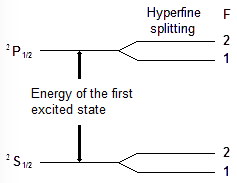
\includegraphics[width=\linewidth]{pictures/hyperfine-splitting.png}
\caption{\textit{Hyperfine splitting energy diagram for I = 3/2 particle
\cite{ref:3}}}
\label{fig:3}
\end{minipage}
\hfill
\begin{minipage}{0.45\linewidth}
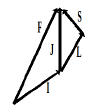
\includegraphics[width=0.3\linewidth]{pictures/hyperfine-vectors.png}
\caption{\textit{Hyperfine coupling in an alkali atom \cite{ref:3}}}
\label{fig:4}
\end{minipage}
\end{figure*}
In the experiment described in this paper we will be studying the absorption 
and emission from Rubidium isotopes (85 and 87) which are alkali atoms. As such the electronic structure of Rubidium is as such,
\begin{equation*}
1s^22s^22p^63s^23p^63d^104s^24p^65s
\end{equation*}
Where we can show the shorthand version as,
\begin{equation*}
[Kr]5s
\end{equation*}
\center
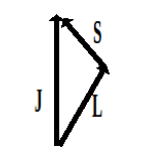
\includegraphics[width=0.3\linewidth]{pictures/electron-angular-momentum.png}
\captionof{figure}{\textit{Coupling of angular momentum in an electron 
\cite{ref:3}.\\}}
\label{fig:1}
\justify
Where, the superscripts show the number of electrons contained in each of the 
electronic shells. Since the only valence electron is in the 5s shell we can 
consider the atom to bev consisting of only one electron. This electron much 
like with other 
electrons can be described by means of the total angular momentum of the 
electron $\vec{J}$ where it is made up of components $\vec{S}$ and 
$\vec{L}$. Which, represent the spin angular momentum and orbital angular 
momentum respectively. The vectors are shown on figure \ref{fig:1}
\\
Since, these components are vectors we can represent the total angular momentum 
as such,
\begin{equation}
\vec{J} = \vec{S}+\vec{L}
\label{eqn:1}
\end{equation}
\justify
Where, for an alkali atom in the ground state the value of $\vec{L}$ is zero 
from the quantum numbers associated with the orbital shell and the value of 
$\vec{S}$ will be 1/2. So, this gives rise to a total angular momentum of 1/2.
\\
As it will later become apparent, we will display some of the energy levels in 
the notation $^{2s+1}L_J$. Where, all of the values are those taken from 
equation \ref{eqn:1}. To represent the ground state of an alkali atom we can 
write it with the formatting $^{2}S_{1/2}$. Since the value of $\vec{L}$ is 
zero by convention we write it as the letter S. Where it to be 1 we would write 
in P and so on.
\\
If the electron were to be in a P state it would be able to have an angular 
momentum of $\vec{L}\pm\vec{S}$ and would take on the representations 
$^{2}P_{1/2}$ and $^{2}P_{3/2}$. Due to the difference in angular momentum the 
energy levels would have different energies. This arises due to the spin-orbit 
coupling of the angular momentum vectors \cite{ref:4}.
\center
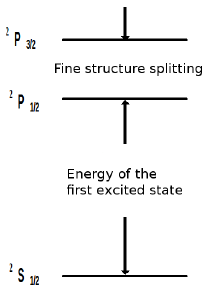
\includegraphics[width=0.5\linewidth]{pictures/energy-levels.png}
\captionof{figure}{\textit{Pictoral representation of the energy difference in the fine structure. Not to scale \cite{ref:3}.}}
\label{fig:2}
\justify
So far, we have been ignoring the effects of the nucleus to make the theory 
easier. However, this will not go on any longer. We will now consider the 
hyperfine splitting of the electron angular momenta. This arises from the 
spin-spin coupling where for the fine structure we had the spin-orbit coupling. 
\\
The spin-spin coupling is due to the magnetic dipole moment of both the proton 
and electron. Now, it should be noted, that the magnetic dipole moment of the 
proton is much smaller than that compared to the electron. The dipole momenta 
can be given as the following.
\begin{equation}
\begin{aligned}
\vec{\mu_p} &= \frac{g_pe}{2m_p}\vec{S_p}
\qquad
\vec{\mu_e} &= -\frac{e}{m_e}\vec{S_e}
\label{eqn:2}
\cite{ref:4}
\end{aligned}
\end{equation}
Where, the p and e represent the proton and electron values respectively, $g_p$ and $g_e$ are the respective g-factors of value 5.59 and 2.00 and $\vec{S}$ 
represents the respective angular spin. Using derivations outlined in reference 
\cite{ref:4} we can get to an expression for the difference in energy of the 
two states with different angular momenta. The equation is as such.
\begin{equation}
\Delta E = \frac{4g_p\hbar}{3m_pm_e^2c^2r^4}
\label{eqn:3}
\cite{ref:4}
\end{equation}
Where, c is the speed of light and r is the radius of the atom. In the 
reference they are making an example to a hydrogen atom with r equal to a 
(Bohr's atomic radius). This derivation can still be generalized to our use as 
we are dealing with an atom that can be approximated to be one that is like a 
hydrogen atom. Where we can also make the relation with the frequency as such.
\begin{equation}
\nu = \frac{\Delta E}{h}
\label{eqn:4}
\cite{ref:4}
\end{equation}
Where the Hamiltonian is as such.
\begin{equation}
H=ha\vec{I}\cdot\vec{J}
\label{eqn:5}
\cite{ref:3}
\end{equation}
Usually the energy difference between these two levels is very small and one 
can cause transitions in the hyperfine structure with an RF wave. A pictoral 
representation of the coupling of the magnetic dipole moment spins is shown on 
figure \ref{fig:4}. Where a rough enegy separation schematic is given in figure 
\ref{fig:3}. As is clearly seen the energy that is required to jump from one 
energy level to the next is muche greater than that required to make the 
transition in the hyperfine structure. Later we will discuss the implications 
of this with respect to optical pumping.
\\
However next we will show another form of splitting where all of the degenerate 
energy levels of the electronic energy level diagram are split.

\subsection{Interaction of an alkali atom with a magnetic field}
\begin{figure*}
\begin{minipage}{0.45\linewidth}
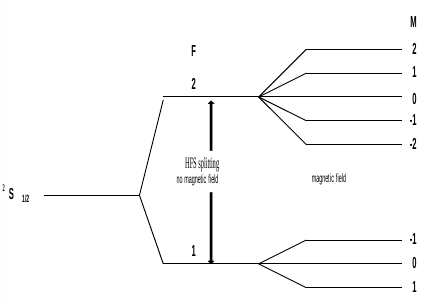
\includegraphics[width=\linewidth]{pictures/zeeman-splitting.png}
\caption{\textit{Energy levels of an alkali atom of the $^2S_{1/2}$ state in a 
weak magnetic field \cite{ref:3}}}
\label{fig:5}
\end{minipage}
\hfill
\begin{minipage}{0.45\linewidth}
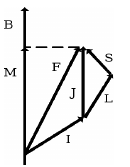
\includegraphics[width=0.3\linewidth]{pictures/zeeman-vectors.png}
\caption{\textit{Zeeman effect in an alkali atom \cite{ref:3}}}
\label{fig:6}
\end{minipage}
\end{figure*}
This interaction is better known as the Zeeman effect and the general premise 
behind this effect is that by applying a magnetic field to an atom we can 
further split the degenerate energy levels according to their angular momenta.
\\
In the Zeeman effect there are three main regions that are to be considered: 
weak field, intermediate and Strong field effects. For the purposes of this 
experiment we will only deal with the weak field effect as the strong field 
can require magnetic fields around 10T which is only achievable with 
extremely expensive equipment.
\\
The Zeeman effect is an effect which can break the spin-orbit coupling of an 
electron creating a difference in energy between the different orbitals of an 
atom. The weak field Zeeman effect is named as such because the energy 
splitting from the Zeeman effect is very small comparatively and as such the 
Hyperfine splittings dominate with the Zeemna effect becoming the pertubation 
\cite{ref:4}. The hamiltonian of this effect is as shown.
\begin{equation}
H=ha\vec{I}\cdot\vec{J}-\frac{\mu_J}{J}\vec{J}\cdot\vec{B}-\frac{\mu_I}{I}\vec{I}\cdot{B}
\label{eqn:6}
\cite{ref:3}
\end{equation}
Where, $\mu_J$ is the electronic dipole moment and $\mu_I$ is the nuclear 
magnetic dipole moment.
\\
Figure \ref{fig:5} shows the energy levels from the weak field Zeeman effect. 
The energy levels are splitting into $2F+1$ levels. Where F is the angular 
momentum of the atom, M is the projection of F onto the direction of the 
magnetic field. In figure \ref{fig:1} we show two levels for the ground state 
and the first excited state. For this experiment we are only considering the 
first excited state $^2P_{1/2}$. The reason why we only consider this and not 
the $^2P_{3/2}$ is because at $\vec{J}$ values of 1/2 we can calculate the 
energy levels in closed form from quantum mechanics with the Breit-Rabi 
equation.
\\
Since the electron can be considered to be a moving charge with charge 1.6e-19 
Coulombs. This magnetic dipole moment has a value that is equal to the Bohr 
Magneton, $\mu_B$. Ignoring the effects of the nucleus we can then represent 
the magnetic energy as \cite{ref:3}.
\begin{equation}
U = \frac{M(\vec{L}+2\vec{S})\cdot\vec{J}}{J^2}\mu_B B = g_J\mu_B M B
\label{eqn:7}
\cite{ref:3}
\end{equation}
Where, $g_J$ is the Lande g-factor which describes the change in the magnetic 
moment of an electron bound in an atom, B is the magnetic field and M is the 
atomic spin component along the magnetic field direction. The g-factor is 
given by,
\begin{equation}
\begin{aligned}
g_J &= \frac{(\vec{L}+2\vec{S})\cdot\vec{J}}{J^2}
\\
g_J &= 1+\frac{J(J+1)+S(S+1)-L(L+1)}{2J(J+1)}
\label{eqn:8}
\cite{ref:3}
\end{aligned}
\end{equation}
To show the interaction energy of an electron we simply need to add a negative 
sign to equation \ref{eqn:7} from the negative charge of the electron. In the 
case of rubidium where we have a J and S value of 1/2 we find that the g-factor 
is equal to 2.00232 \cite{ref:3}.
\\
Now, if we were to include the iteraction of the nucleus to find the 
interaction energy the equation could be represented as follows.
\begin{equation}
U = -g_F\mu_B M B
\label{eqn:9}
\cite{ref:3}
\end{equation}
Where, $g_F$ can be shown to be the following.
\begin{equation}
g_F = g_J\frac{F(F+1)+J(J+1)-I(I-1)}{2F(F+1)}
\label{eqn:10}
\cite{ref:3}
\end{equation}
Where, F represents the total angular momentum of the atom, I is the total 
nuclear spin angular momentum and J is the total electronic angular momentum. 
This quantity is highly dependent on the atom that is being used and as such 
there is no one set value as with the Lande g-factor.
\\
the above equations are only applicable when the interaction energy with the 
magnetic field is very small and depends linearly. If the dependence is 
quadratic, which will be studied in this experiment, we must apply the 
Breit-Rabi equation which can be derived by diagonalizing the Hamiltonian in 
equation \ref{eqn:6} \cite{ref:3}. The result of such is the following.
\begin{equation}
\begin{aligned}
W(F,M) = -&\frac{\Delta W}{2(2I+1)}-\frac{\mu_I}{I}MB\pm ...
\\
          &\frac{\Delta W}{2}\left[1+\frac{4M}{2I+I}x+x^2\right]^{1/2}
\label{eqn:11}
\cite{ref:3}
\end{aligned}
\end{equation}
Where,
\begin{equation}
x = (g_J - g_I)\frac{\mu_B B}{\Delta W}
\label{eqn:12}
\cite{ref:3}
\end{equation}
\begin{equation}
g_I = -\frac{\mu_I}{I\mu_B}
\label{eqn:13}
\cite{ref:3}
\end{equation}
\begin{figure*}
\begin{minipage}[t]{\textwidth}
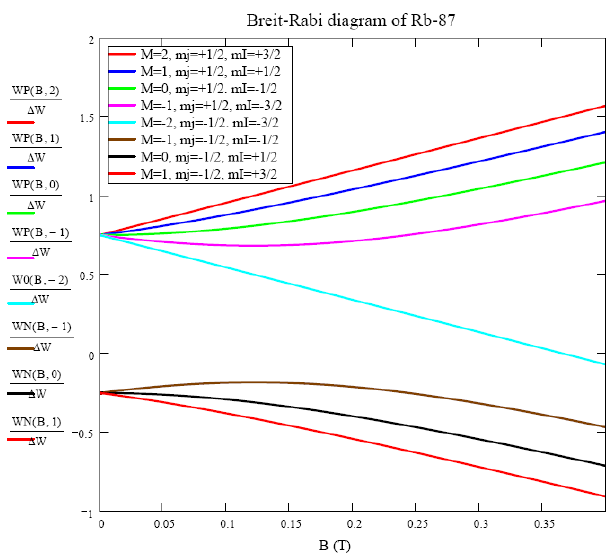
\includegraphics[width=\linewidth]{pictures/breit-rabi.png}
\caption{\textit{Breit-Rabi diagram of $Rb^{87}$ in a magnetic field \cite{ref:3}.}}
\label{fig:7}
\end{minipage}
\end{figure*}
Where, W is the interaction energy and $\Delta$W is the hyperfine splitting 
energy.
\\
Figure \ref{fig:7} shows a plot of the Breit-Rabi equation. The three Zeeman 
levels for the magnetic field are as follows. Weak field is at an x value close 
to zero where the energy splitting varies linearly and the hyperfine 
interaction dominates where the Zeeman effect is the pertubation. The strong 
field region, also known as the Paschen-Back region is x values greater than 2 
where the energy levels are linear once again and depends on the Zeeman effect 
where the hyperfine splitting is taken as the pertubation. The final region 
is the intermediate field region at values greater than zero but less than 2. 
In this region both the hyperfine splitting and the Zeeman effect contribute 
equally to the energy splitting of the electronic orbitals \cite{ref:4}.
\\
In this experiment we are only concerned with the weak field Zeeman effect.

\subsection{Photon absorption in an alkali atom}
\begin{figure*}
\begin{minipage}[t]{\textwidth}
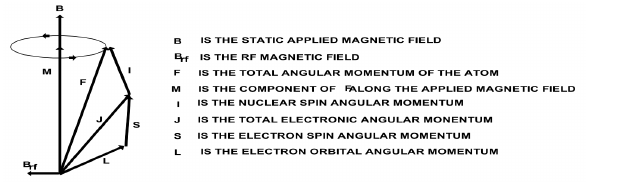
\includegraphics[width=\linewidth]{pictures/all-vectors.png}
\caption{\textit{Magnetic fields and angular momenta involved in the experiment 
\cite{ref:3}.}}
\label{fig:8}
\end{minipage}
\end{figure*}
The lowest electronic state along with the first two excited states of the 
valence electron for a rubidium atom are the following: $^2S_{1/2}$, 
$^2P_{1/2}$ and $^2P_{3/2}$. Where, we will mainly deal with the ground state 
and the first excited state for simplicity.
\\
The transitions from the ground state to the excited state are governed by 
selection rules that are as follows: $\Delta$L = 0,$\pm$1, $\Delta$S = 0 and 
$\Delta$J = 0,$\pm$1. However, the value of L cannot go from 0 to 0 
\cite{ref:3}.
\\
For this experiment we are interested in the amount of light that is absorbed 
or transmitted by the rubidium atoms in a given volume. For this purpose it can 
be useful to use the concept of a cross section of the atoms. In the limit of 
low density this can be represented as.
\begin{equation}
n = n_0e^{-\sigma\rho l}
\label{eqn:14}
\cite{ref:3}
\end{equation}
Where, n and n$_0$ are the incoming and outgoing flux of electrons and $\rho$ 
is the density of the gas.
\\
A similar concept can be employed when talking about a flux of photons.
\begin{equation}
I = I_0 e^{-\sigma_0\rho l}
\label{eqn:15}
\cite{ref:3}
\end{equation}
Where the cross section in this equation is actually the cross section at the 
resonance condition which is much lower than the expected value.
\\
Now we must append to our selection rules for transitions to account for the 
selection rules for the hyperfine splitting which will add that $\Delta$F = 
0,$\pm$1. Additional splitting caused by the magnetic field adds that $\Delta$M 
= 0,$\pm$1.
\\
The selection rule for M can be somewhat different, because since angular 
momentum must always be conserved the absorption of light must be circularly 
polarized. Of course, if light is circularly polarized we will be adding to 
the angular momentum. The question then becomes how does it change depending on 
the polarization.
\\
It has already been established that only circularly polarized will change the 
angular momentum of the atom. So, depending on the polarization we will get 
addition or subtraction to the angular momentum. That is to say that we will 
have either a +1 or a -1 to the angular momentum, never both.
\\
The lifetime of the transitions will be determined by collision processes. 
It is mentioned that the rubidium glass bulb is filled with a buffer gas that 
is there to decrease the collisions of the atoms with the walls of the 
container and lose its angular momentum. The neon gas dissaallows this from 
happening and since it is a very symmetric atom it will not contribute much to 
the decrease of the angular momentum of the atom \cite{ref:1}.

\subsection{Optical pumping in rubidium}
\begin{figure*}
\begin{minipage}[t]{\textwidth}
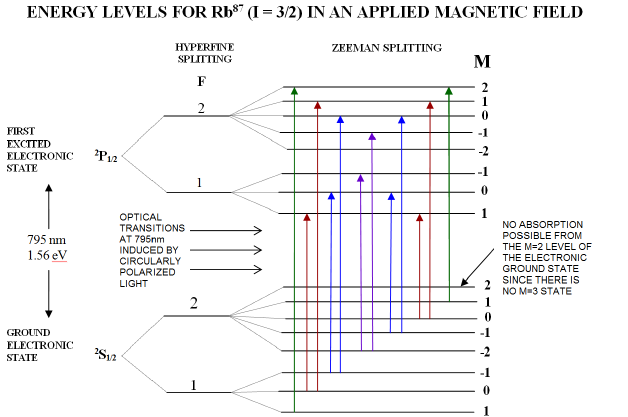
\includegraphics[width=\linewidth]{pictures/energy-lev-trans.png}
\caption{\textit{Transitions involved in the optical pumping of $Rb^{87}$ 
\cite{ref:3}.}}
\label{fig:8}
\end{minipage}
\end{figure*}
In optical pumping we are trying to drive for there to be a net population 
difference in one state relative to another. On figure \ref{fig:8} we see the 
types of transitions that are possible. On the left side of the figure we see 
that there is a large separation between the energy levels that corresponds to 
a transition energy of a 795 nm photon.
\\
In order to create this 795 nm photon an RF discharge lamp is used to create 
circulary polarized light at that wavelength. Inside it there is rubidium gas 
and when it spontaneously emmits light it creates light at 795 and 780 nm. 
By filtering out the 780 nm photons we get a circularly polarized 795 nm photon 
beam.
\\
On the right side of figure \ref{fig:8} we see the electronic levels from the 
Zeeman splitting. The transitions between these energy levels are caused by the 
RF magnetic field that runs perpendicular to the permanent coil.
\\
After sufficient time is allowed for the transitions to be carried out it can 
be seen that there will be a population on the M = 2 level since the circularly 
polarized light will add angular momentum to the electrons on the orbital 
levels and 

\begin{thebibliography}{9}
\bibitem{ref:1}
Bloom, A L (1960). Optical Pumping. \emph{Scientific American} October, 72.
\bibitem{ref:2}
Benumof, R (1965). Optical Pumping Theory and Experiments. \emph{American 
Journal of Physics 33}, 151.
\bibitem{ref:3}
UB 2015 Lab Manual. Optical Pumping.
\bibitem{ref:4}
Griffiths, D J (2005). Introduction to Quantum Mechanics. Upper Saddle river, 
New Jersey: \emph{Pearson Prentice Hall}.

\end{thebibliography}

\end{document}
